% ++++++++++++ Domain Pi AKS klassen ++++++++++++++
\subsubsection{Domain-klasse: Aks}

\begin{figure}[h]
\centering
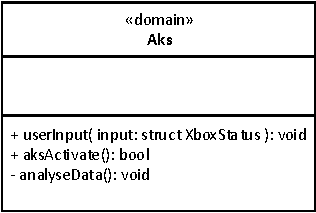
\includegraphics[]{../fig/diagrammer/bil/cd_aks.pdf}
\caption{Klassebeskrivelse for domain-klassen Aks}
\label{fig:cd_aks}
\end{figure}

\textbf{Attributter}

\begin{table}[h]
\begin{tabularx}{\textwidth}{| Z | Z | L{10cm} |} \hline
Navn & Type & Beskrivelse \\\hline
\texttt{MySteering} & \texttt{Steering} & Styretøjsklassen, bruges når Aks skal påvirke bilens hastighed eller retning.\\\hline
\texttt{MyData} & \texttt{Data*} & Pointer til bilens datastruktur.\\\hline
\end{tabularx}
\caption{Attributter for klassen Aks}
\label{table:attr_aks}
\end{table}

\textbf{Metoder}

%----------------- userInput -------------------

\begin{table}[h]
\begin{tabularx}{\textwidth}{| L{2.5 cm} | Z |} \hline
Prototype & \texttt{void userInput(XboxStatus input)} \\\hline
Parametre & \texttt{input} \newline En struct med alle input fra brugeren. \\\hline
Returværdi &  \texttt{void} \\\hline
Beskrivelse & Metoden sender input fra brugeren videre til Steering-klassen. \\\hline
\end{tabularx}
\caption{Metodebeskrivelse for \texttt{userInput}}
\label{table:met_aks_userInput}
\end{table}

%----------------- aksActivate -------------------
\begin{table}[h]
\begin{tabularx}{\textwidth}{| L{2.5 cm} | Z |} \hline
Prototype & \texttt{void aksActivate(void)} \\\hline
Parametre & \texttt{void}  \\\hline
Returværdi &  \texttt{bool} \newline Returnerer \texttt{TRUE} hvis det gik godt og \texttt{FALSE} hvis der skete fejl undervejs. \\\hline
Beskrivelse & Metoden kaldes når det automatiske anti-kollisionssystem skal aktiveres. Forhindrer samtidigt input fra brugeren kortvarigt. \\\hline
\end{tabularx}
\caption{Metodebeskrivelse for \texttt{aksActivate}}
\label{table:met_aks_aksActivate}
\end{table}

%----------------- analyseData -------------------
\begin{table}[h]
\begin{tabularx}{\textwidth}{| L{2.5 cm} | Z |} \hline
Prototype & \texttt{void analyseData(void)} \\\hline
Parametre & \texttt{void}  \\\hline
Returværdi &  \texttt{void}  \\\hline
Beskrivelse & Metoden analyserer indhentet data fra Data klassen og vurderer hvilken type af undvigelse der bedst passer. Aktiverer herefter Steering-klassen for at bilen skal undvige forhindringen. \\\hline
\end{tabularx}
\caption{Metodebeskrivelse for \texttt{analyseData}}
\label{table:met_aks_analyseData}
\end{table}